
\section{Characterizing Limitations of Monotonic Factorization}
Monotonic factorization restricts the family of global action value functions that can be represented. More precisely, 
$Q_{tot}(\mathbf{s}, \boldsymbol{u}) = f_\theta(\mathbf{s}, Q_1(\tau_1, u_1), ..., Q_n(\tau_n, u_n))$ implies that if $u_1^* = \text{argmax} Q_1(\tau_1, u_1)$ is the optimal action choice for agent 1, $u_1^*$ must also be optimal for all other states with varying $\tau_2,\ldots,\tau_n$. We analyze this restriction and show how it makes monotonic factorization ineffective in representing complex global value functions.


Considering a Markov decision process (MDP) with $n$ agents, where the state of agent $i$ is denoted by $s_i \in S$ and action by $u_i \in A$, for $i = 1, 2, ..., n$, composing a joint state $\textbf{s}$ and joint action $\textbf{u}$. Let $Q_i(s_i, u_i)$ be local agent value utilities, $Q_{jt}(\mathbf{s}, \textbf{u})$ be the unrestricted ground truth of joint action-value function, and $Q_{mono}(\mathbf{s}, \textbf{u})$ be an arbitrary monotonic factorization estimate of $Q_{jt}(\mathbf{s}, \textbf{u})$. Ideally, the monotonic factorization estimate $Q_{mono}$ should be able to recover the exact optimal action selections of $Q_{jt}$. We define $S_{mono}$ as the state set, where $Q_{mono}$ and $Q_{jt}$ have the same optimal joint action, i.e., 
\begin{eqnarray}
S_{mono}=\left\{ \mathbf{s}: \arg\max Q_{mono}(\mathbf{s}, \textbf{u}) = \arg\max  Q_{jt}(\mathbf{s}, \textbf{u}) \right\} \nonumber
\end{eqnarray}
We show that $|S_{mono}|$ can be arbitrarily small compared to the state space $|S|^n$, when the global maximums are uniformly distributed in  $Q_{jt}(\mathbf{s}, \textbf{u})$. Thus, monotonic factorization could only recover an arbitrarily small fraction of action choices.


{
\begin{theorem}
 When $n \geq log_{|S|}(2|A|\cdot log_2|A|) + 1$ and the optimal action choices in $Q_{jt}$ are uniformly distributed, for any monotonic factorization, we have
$\frac{E(|S_{mono}|)}{|S|^n} \leq \frac{e+1}{|A|}\cdot \delta^{n-1}$ for some constant $\delta\in(0,1)$.
\end{theorem}



\noindent\textbf{Proof  Sketch.} We give a sketch of the proof and provide the complete proof in Appendices. Our key idea is to convert the problem into a classic max-load problem~\cite{balls_into_bins}.

\noindent \textit{\textbf{Step1}: Formulate as max-load bin-ball problem.} For each agent $i$ and state $\mathbf{s}$, we consider the optimal action of $Q_{mono}$ as \textit{ball $i$}. Thus, $Q_{jt}$ and $Q_{mono}$ have the same optimal action for agent $i$ if ball $i$ is placed in the bin corresponding to the optimal action of $Q_{jt}$. 

%the \textit{bin $i$} is the optimal action of $Q_{jt}$.

Let $X_i$ denotes that ball $i$ is in bin $i$, that is,  $Q_{jt}$ and $Q_{mono}$ have the same optimal action for  agent $i$, then we have: 
%. Our goal is to analyze $max_{1 \leq  i \leq n}Xi$
\begin{equation}
    E(|S_{mono}|) = \Sigma_sP(X_1)\cdot P(X_2|X_1) \cdot...\cdot P(X_n|X_{n-1}...X_1) \nonumber
\label{S_mono}
\end{equation}

Define $Y_i$ as the load of bin $i$, that is, the state space such that $Q_{jt}$ and $Q_{mono}$ have the same optimal action for agents except for agent $i$.
Note that the global maximum of $Q_{jt}$ is uniformly distributed over different states, we then analyze $P(X_1)$:
\begin{equation}
P(X_1) =  \frac{E(\Sigma_{s_2...s_n}X_1)}{|S|^{n-1}}
\leq \frac{E(max_{i}Y_i)}{|S|^{n-1}}
\label{P_X_1}
\end{equation}

\noindent \noindent\textit{\textbf{Step2}: Analyze the probability distribution of the load.} According to the Chernoff bound and the Union bound, we have: when $n \geq log_{|S|}(2|A|\cdot log_2|A|) + 1$,
\begin{equation} 
E(max_{i}Y_i) \leq \frac{(e+1) \cdot {|S|^{n-1}}}{|A|}.
\label{maxY}
\end{equation}
where $|A| \geq 1$ is the size of action space. 

Applying Eq. (\ref{maxY}) to Eq. (\ref{P_X_1}) and Eq. (\ref{S_mono}), we have:
\begin{equation}
P(X_1) \leq \frac{e+1}{|A|}
\end{equation}
Using the same argument repeatedly for agents $i=2,\ldots,n$, we can choose $\delta = min_i(P(X_i|X_{i-1}...X_1))$ and $0 < \delta < 1$. Plugging these inequalities into $ E(|S_{mono}|) $, it yields the desired result $\frac{E(|S_{mono}|)}{|S|^n} \leq \frac{e+1}{|A|}\cdot \delta^{n-1}$.

\iffalse
 \begin{equation}

E(|S_{mono}|) \leq \frac{e+1}{|\overline{u}|}\cdot \delta^{n-1} \cdot |S|^n
\end{equation}
where $\delta = min_i(P(X_i|X_{i-1}...X_1)$ and $0 < \delta < 1$.


\noindent\textit{\textbf{Step3}: Calculate the upper bound of the fraction}
The final fraction of $E(|S_{mono}|)$ over the overall state space satisfies:
 \begin{equation}
\frac{E(|S_{mono}|)}{|S|^n} \leq \frac{e+1}{|\overline{u}|}\cdot \delta^{n-1}
\end{equation}
when $n \geq log_{|S|}(2|\overline{u}|\cdot log_2|\overline{u}|) + 1$.

\fi


\begin{figure*}[ht!]
\centering
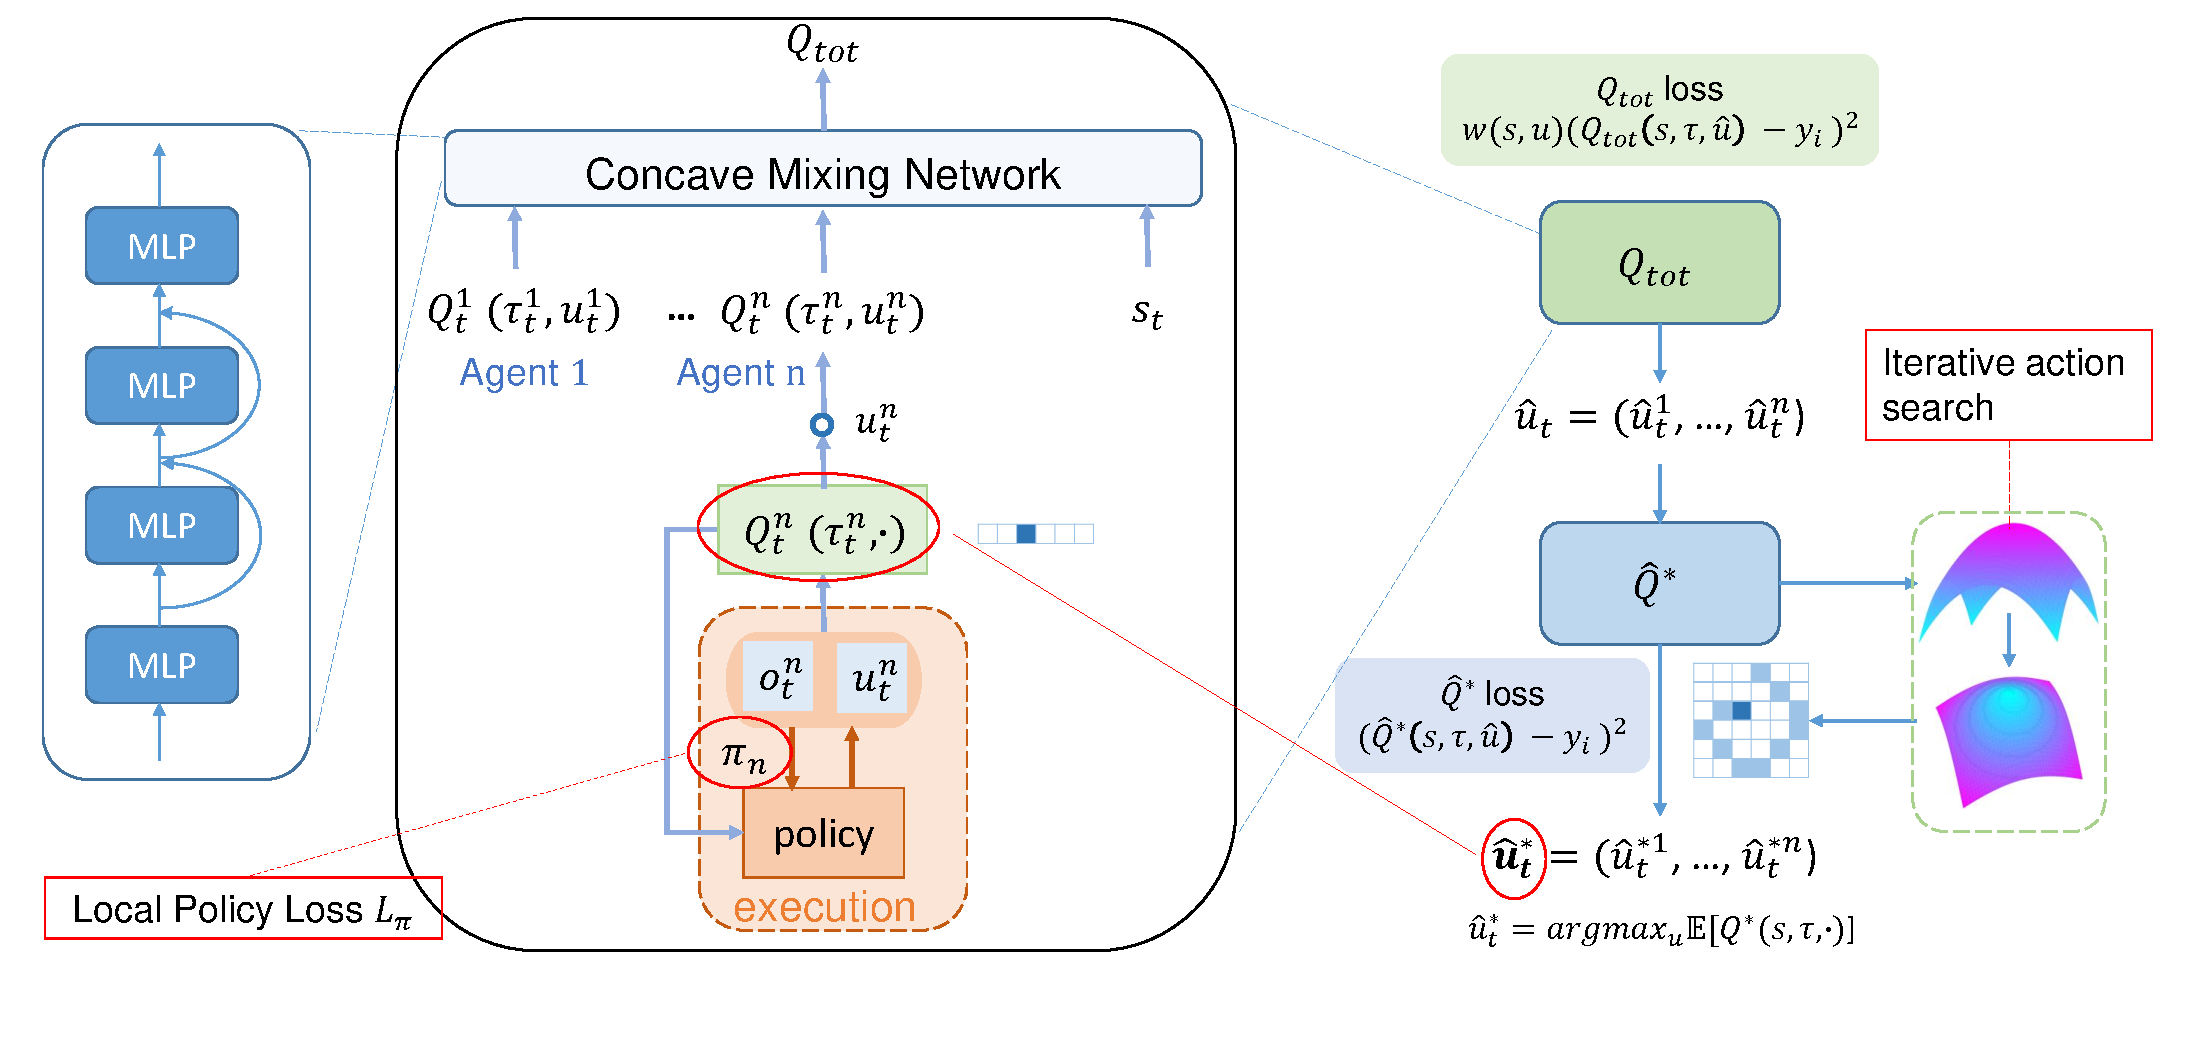
\includegraphics[scale=0.4]{new_figure/framework_v8.pdf}
\caption{The overall architecture of ConcaveQ. The concave mixing network represents $Q_{tot}$ as a concave function of local $Q_a$. With the help of iterative action selection, we can select the optimal actions during training. As for the execution process, the soft policy network is used to find the optimal actions. }
\label{framework}
\end{figure*}


Our analysis shows that a monotonic mixing can only recover an arbitrarily small fraction of global value function maximums, as the number of agents or the size of action space increases. 
%Moreover, as the number of agents becomes sufficiently large, this fraction can be arbitrarily small.} 
Our proposed ConcaveQ addresses the representation issue by introducing a concave mixing network to value function factorization, to enhance the representation ability for better performance. Since the IGM principle no longer holds under concave mixing functions, the greedy action selection by maximizing local agent Q values can not be adopted.
Note that concave optimization has good convergence properties \cite{concaveopt}, that is, a concave function has only one global maximum and the maximum can always be obtained using iterative methods. Therefore,  ConcaveQ tackles the action selection problem by optimizing the joint value function in an iterative manner. As for execution, note that the optimal joint action cannot be obtained directly from maximizing the local agent $Q_i$, we adopt a soft actor-critic policy network in ConcaveQ that uses factorized policies to support distributed execution, such that each local agent can select the best action according to its own local policy network which will be corrected by the Concave value networks during training while exploiting auxiliary information for learning. Moreover, entropy maximization is also used to enhance effective exploration.  As for concave mixing networks, there is always a concave mixing way that can recover the global maximum. 
 
{\begin{prop}
For any state $s$, there is always a concave function $Q_{c}(s, \textbf{u})$ that recovers the global maximum of  $Q_{jt}(s, \textbf{u})$ with the same optimal action.
\end{prop}  

\noindent\textbf{Proof  Sketch.\ } 
For any state $s$, let $f_1(\textbf{u})$ = $Q_{jt}(, \textbf{u})$ and $f_2(\textbf{u})$ = -$Q_{jt}(, \textbf{u})$. According to Fenchel–Moreau theorem \cite{convex_conjugate}, the biconjugate function of $f_2(\textbf{u})$ is a convex function $g(\textbf{u}) = f_2^{**}(\textbf{u})$ and $h(\textbf{u}) = -f_2^{**}(\textbf{u})$  is a concave function. $g(\textbf{u})$ and $h(\textbf{u})$ satisfies:
 \begin{equation}
    g(\textbf{u}) \leq f_2(\textbf{u}), 
\end{equation}
 \begin{equation}
    h(\textbf{u}) \geq f_1(\textbf{u}).
\end{equation}
Suppose the optimal joint action of $f_1(\textbf{u})$ and $h(\textbf{u})$ are $\textbf{u}_{f_1}^*$ and $\textbf{u}_h^*$ respectively,  if we shift $h(\textbf{u})$ by $(-\textbf{u}_{f_1}^* + \textbf{u}_h^*)$, the shifted concave function has the same optimal action as $f_1(\textbf{u})$. In other words, for any state $s$, there is always a concave function that has the same optimal action as $Q_{jt}(s, \textbf{u})$. 
}

The key to our method is the insight that it is not necessary to use the monotonic factorization of QMIX  to extract decentralized policies that are fully consistent with their centralized counterpart. Next, we will discuss concave mixing network design and our ConcaveQ framework to support fully decentralized execution.
